\documentclass{ximera}

%\addPrintStyle{..}

\begin{document}
	\author{Bart Lambregs}
	\xmtitle{Relatie met een cirkelbeweging}{}
    \xmsource\xmuitleg



	%%%\section{Relatie met een cirkelbeweging}

	Wanneer we op een grammofoonplaat en klein object leggen en met een lamp de schaduw op de muur bekijken terwijl de plaat draait, dan zien we evenzeer een op- en neergaande beweging. 
	\begin{image}
	%
	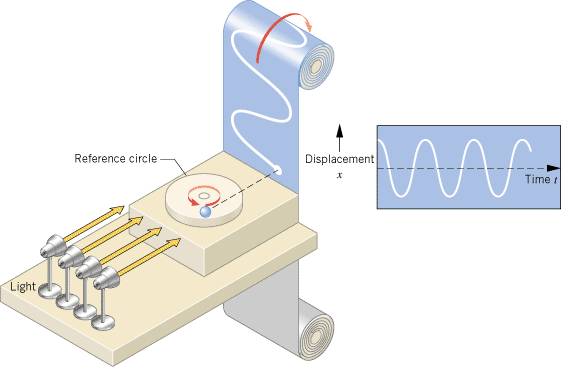
\includegraphics[width=.6\textwidth]{ht_schaduw}
	\hspace{5mm}
	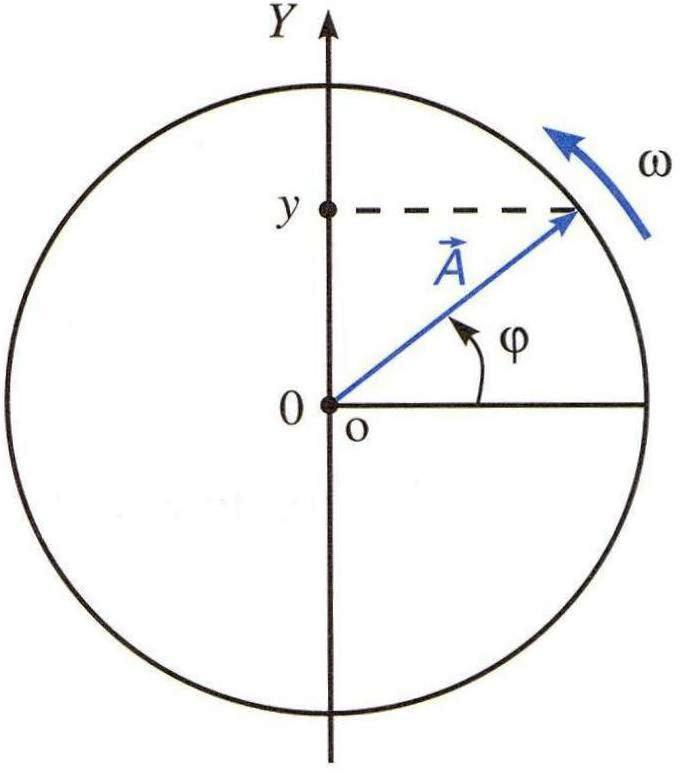
\includegraphics[width=.35\textwidth]{fasor}
	\end{image}
	Het gaat hier echter ook om een harmonische trilling. Bekijken we immers de $y$-coördinaat van een punt op een cirkel dat met een constante hoeksnelheid beweegt, dan is dit een sinusfunctie. Als we bovendien de hoeksnelheid van de cirkelbeweging gelijk nemen aan de pulsatie van een harmonische trilling, de straal even lang maken als de amplitude en op tijdstip $t=0$ het punt op de cirkel een omwentelingshoek $\varphi$ geven, dan beschrijft de $y$-coördinaat eenzelfde harmonische trilling. 
	
	De plaatsvector die het punt op de cirkel beschrijft noemen we ook wel een \emph{fasor} -- een samenvoegsel van fase en vector. Met een fasor kunnen de fase van een trilling visualiseren, het faseverschil tussen trillingen visualiseren en kunnen we gemakkelijker trillingen samenstellen. 
	
	%%%\newpage
	

\end{document}
